\section{Data and Preprocessing}
\subsection{Dataset}
The Fashion-MNIST is a dataset of Zalando article images, consisting of a training set of 60,000 samples and 10,000 test samples.
The dataset used here is a small portion of the original dataset, 10,000 training and 5,000 test samples.
Each sample is a 28x28 pixels gray-scale image with a label indicating the type of clothing item associated with each.
\newline

\begin{figure}[ht]
\centering
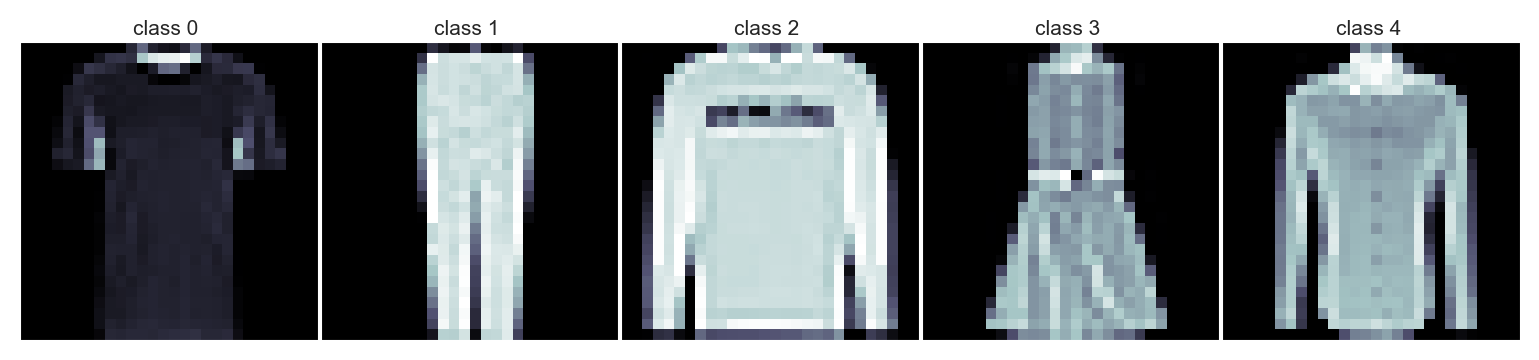
\includegraphics[scale=0.45]{figures_for_report/samples_from_classes}
\captionsetup{justification=centering,margin=2cm}
\caption{One sample from each class}
\end{figure}\\

Table 1 shows the translation from class labels to clothing type.
The clothing type will be used instead of the labels in the report for better readability \\
\begin{table}[!ht]
  \footnotesize
  \centering
\begin{tabular}{ c c c c c c }
 \toprule
 \textbf{Label} & 0 & 1 & 2 & 3 & 4 \\
 \midrule 
 \textbf{Type of clothing} & T-shirt/Top & Trousers & Pullover & Dress & Shirt \\
 \bottomrule
\end{tabular} \\[0.2cm]
\captionsetup{justification=centering,margin=2cm}
\caption{Mapping from class-labels to clothing type}
\label{tab:features}
\end{table}


\subsection{Data Cleaning}\label{subsec:data-cleaning}
The dataset provided was already in a cleaned state, which was verified by checking for missing values,
and checking that the pixel values were no greater than 255 and no smaller than 0.

\subsection{Preprocessing}\label{subsec:preprocessing}
The pixels values were in the range $[0, 255]$.
This range was normalized to $[0, 1]$ by dividing each pixel by 255.
This was done to improve training time and make it easier for neural networks to work with the data, as smaller numbers are slightly faster to compute and are preferred by neural networks


\subsection{Class Distribution}\label{subsec:class-distribution}
Whether or not a machine learning model can learn to predict classes well depends to a high degree on how those classes are distributed within our training and training dataset.
Both the datasets are extremely balanced, with the test being fully balanced ($1000$ of each class).
This is illustrated on the plots below

\begin{figure}[ht]
\centering
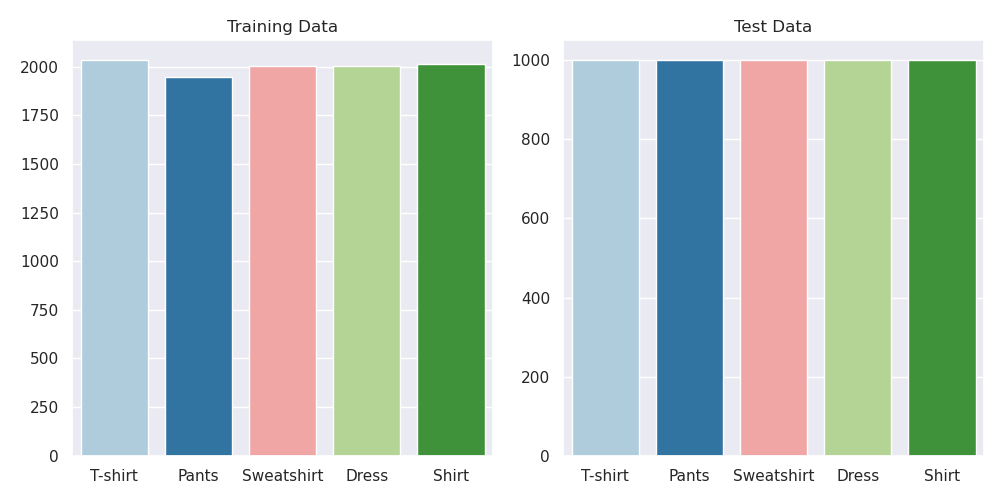
\includegraphics[scale=0.45]{figures_for_report/class_distribution}
\captionsetup{justification=centering,margin=2cm}
\caption{Distribution of clothing items in our training and test dataset}\label{fig:figure2}
\end{figure}

